\let\lesson\undefined
\newcommand{\lesson}{\phantomlesson{Bài 4.}}


\setcounter{section}{2}
\section{Bài tập trắc nghiệm}
\begin{enumerate}[label=\bfseries Câu \arabic*:,leftmargin=1.5cm]
	\item \mkstar{1}\\
	Đại lượng đặc trưng cho tính chất nhanh hay chậm của chuyển động là 
	\begin{mcq}(4)
		\item toạ độ.
		\item gia tốc.
		\item quãng đường đi.
		\item tốc độ.
	\end{mcq}
\hideall{
\textbf{Đáp án D.}
}

\item \mkstar{1}\\
Khi nhìn vào tốc kế của ô tô đang chạy, số chỉ trên tốc kế cho ta biết
\begin{mcq}(2)
	\item gia tốc tức thời của ô tô.
	\item vận tốc tức thời của ô tô.
	\item tốc độ tức thời của ô tô.
	\item tốc độ trung bình của ô tô.
\end{mcq}
\hideall{
\textbf{Đáp án C.}
}

\item \mkstar{2}\\
Một máy bay phản lực có tốc độ $\SI{700}{\kilo\meter/\hour}$. Nếu muốn bay liên tục trên khoảng cách $\SI{1400}{\kilo\meter}$ thì máy bay phải bay trong thời gian là
\begin{mcq}(4)
	\item $\SI{2}{\hour}$.
	\item $\SI{3}{\hour}$.
	\item $\SI{2}{\hour}\SI{30}{\minute}$.
	\item $\SI{1}{\hour}\SI{30}{\minute}$.
\end{mcq}
\hideall{
\textbf{Đáp án A.}\\
Thời gian máy bay bay quãng đường $\SI{1400}{\kilo\meter}$:
$$t=\dfrac{s}{v}=\SI{2}{\hour}.$$
}

\item \mkstar{2}\\
Một xe xuất phát từ lúc 7 giờ 15 phút sáng từ thành phố M, chuyển động thẳng đều tới thành phố N, cách thành phố M $\SI{90}{\kilo\meter}$. Biết tốc độ của xe là $\SI{60}{\kilo\meter/\hour}$, xe đến thành phố N lúc
\begin{mcq}(4)
	\item 9 giờ 45 phút.
	\item 8 giờ 30 phút.
	\item 9 giờ 30 phút.
	\item 8 giờ 45 phút.
\end{mcq}
\hideall{
\textbf{Đáp án D.}\\
Thời gian để xe đi từ M đến N:
$$\Delta t=\dfrac{s}{v}=\SI{1.5}{\hour}.$$
Thời điểm xe đến N:
$$t=\SI{7}{\hour}\SI{15}{\minute}+\Delta t=\SI{8}{\hour}\SI{45}{\minute}.$$
}

\item \mkstar{2}\\
Một vận động viên chạy cự li $\SI{600}{\meter}$ mất $\SI{74.75}{\second}$. Hỏi vận động viên đó có tốc độ trung bình bao nhiêu?
\begin{mcq}(4)
	\item $\SI{8.03}{\meter/\second}$.
	\item $\SI{9.03}{\meter/\second}$.
	\item $\SI{10.03}{\meter/\second}$.
	\item $\SI{11.03}{\meter/\second}$.
\end{mcq}
\hideall{
\textbf{Đáp án A.}\\
Tốc độ trung bình của vận động viên:
$$v_\text{tb}=\dfrac{s}{\Delta t}=\SI{8.03}{\meter/\second}.$$
}

\item Trong nội dung thi đấu môn bơi ếch $\SI{100}{\meter}$, một vận động viên đã hoàn thành đường đua với thành tích $\SI{63.25}{\second}$. Tốc độ trung bình của vận động viên này trong giải thi đấu đó là bao nhiêu?
\begin{mcq}(4)
	\item $\SI{1.58}{\meter/\second}$.
	\item $\SI{0.63}{\meter/\second}$.
	\item $\SI{6.33}{\meter/\second}$.
	\item $\SI{36.75}{\meter/\second}$.
\end{mcq}
\hideall{
\textbf{Đáp án A.}\\
 Tốc độ trung bình của vận động viên này
 $$v_\text{tb}=\dfrac{s}{t}\approx\SI{1.58}{\meter/\second}.$$
}

\item Một ô tô chạy thử nghiệm trên một đoạn đường thẳng. Cứ $\SI{5}{\second}$ thì có một giọt dầu từ động cơ của ô tô rơi thẳng xuống mặt đường. Hình bên cho thấy mô hình các giọt dầu để lại trên mặt đường. Ô tô chuyển động trên đường này với tốc độ trung bình là
\begin{center}
	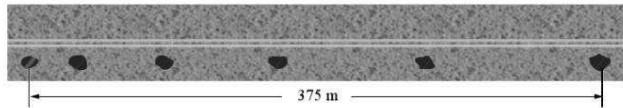
\includegraphics[width=0.5\linewidth]{../figs/VN10-2022-PH-TP004-1-P-1}
\end{center}
\begin{mcq}(4)
	\item $\SI{12.5}{\meter/\second}$.
	\item $\SI{15}{\meter/\second}$.
	\item $\SI{30}{\meter/\second}$.
	\item $\SI{25}{\meter/\second}$.
\end{mcq}
\hideall{
\textbf{Đáp án B.}\\
Tốc độ trung bình của ô tô:
$$v_\text{tb}=\dfrac{s}{t}=\dfrac{\SI{375}{\meter}}{\SI{25}{\second}}=\SI{15}{\meter/\second}.$$
}
	
	\item \mkstar{2}\\
	Một chiếc xe ô tô xuất phát từ A lúc 6 giờ sáng, chuyển động thẳng đều tới B, cách A $\SI{120}{\kilo\meter}$. Biết xe tới B lúc 8 giờ 30 phút sáng, tốc độ trung bình của xe là 
	\begin{mcq}(4)
		\item $\SI{48}{\kilo\meter/\hour}$.
		\item $\SI{45}{\kilo\meter/\hour}$.
		\item $\SI{60}{\kilo\meter/\hour}$.
		\item $\SI{50}{\kilo\meter/\second}$.
	\end{mcq}
\hideall{
	\textbf{Đáp án A.}\\
	Tốc độ trung bình của xe:
	$$v_\text{tb}=\dfrac{s}{t_2-t_1}=\SI{48}{\kilo\meter/\hour}.$$
}

	\item \mkstar{3}\\
	{Một xe chuyển động thẳng không đổi chiều, $\SI{1}{\hour}$ đầu xe chạy với tốc độ trung bình $\SI{60}{\kilo\meter/\hour}$ và $\SI{3}{\hour}$ sau xe chạy với tốc độ trung bình $\SI{40}{\kilo\meter/\hour}$. Tính tốc độ trung bình của xe trong suốt thời gian chuyển động.
		\begin{mcq}(4)
			\item $\SI{48}{\kilo\meter/\hour}$.
			\item $\SI{40}{\kilo\meter/\hour}$.
			\item $\SI{58}{\kilo\meter/\hour}$.
			\item $\SI{45}{\kilo\meter/\hour}$.
		\end{mcq}
	}
	\hideall{
		\textbf{Đáp án: D.}\\
		$$v_{tb}=\dfrac{v_1t_1+v_2t_2}{t_1+t_2}=\SI{45}{\kilo\meter/\hour}.$$
	}
	
	\item \mkstar{3}\\
	{Một người đi xe đạp trên $\dfrac{2}{3}$ đoạn đường đầu với tốc độ trung bình $\SI{10}{\kilo\meter/\hour}$ và $\dfrac{1}{3}$ đoạn đường sau với tốc độ trung bình $\SI{20}{\kilo\meter/\hour}$. Tốc độ trung bình của người đi xe đạp trên cả quãng đường là
		\begin{mcq}(4)
			\item $\SI{12}{\kilo\meter/\hour}$.
			\item $\SI{15}{\kilo\meter/\hour}$.
			\item $\SI{17}{\kilo\meter/\hour}$.
			\item $\SI{13.3}{\kilo\meter/\hour}$.
		\end{mcq}
	}
	\hideall{
		\textbf{Đáp án: A.}\\
		Gọi $s$ là chiều dài đoạn đường
		$$v_{tb}=\dfrac{s}{t_1+t_2}=\dfrac{s}{\dfrac{2s}{3v_1}+\dfrac{s}{3v_2}}=\dfrac{1}{\dfrac{2}{3v_1}+\dfrac{1}{3v_2}}=\SI{12}{\kilo\meter/\hour}.$$
	}
\end{enumerate}
\section{Bài tập tự luận}
\begin{enumerate}[label=\bfseries Bài \arabic*:,leftmargin=1.5cm]
	\item \mkstar{2}\\
	{		Hãy tính tốc độ trung bình ra m/s và km/h của nữ vận động viên tại một số giải thi đấu dựa vào bảng:
		\begin{center}
			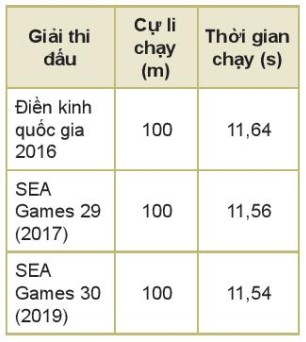
\includegraphics[width=0.3\linewidth]{../figs/VN10-2022-PH-TP005-5.jpg}
		\end{center}
	}
	\hideall
	{		Tốc độ trung bình của nữ vận động viên tại giải điền kinh quốc  gia 2016 là:
		$$v_\text{tb} = \dfrac{s}{t} =\dfrac{100}{\SI{11,64}{}} = \SI{8,6}{m/s} = \SI{30,96}{km/h}.$$
		Tốc độ trung bình của nữ vận động viên tại SEA GAME 19, 2017  là 100 : 
		$$v_\text{tb} = \dfrac{s}{t} =\dfrac{100}{\SI{11,56}{}} = \SI{8,65}{m/s} = \SI{31,141}{km/h}.$$
		Tốc độ trung bình của nữ vận động viên tại SEA GAME 30, 2019 là 100: 
		$$v_\text{tb} = \dfrac{s}{t} =\dfrac{100}{\SI{11,54}{}}= \SI{8,66}{m/s} = \SI{31,195}{km/h}.$$
	}

	\item \mkstar{2}
	
	
	{
		Một người đi xe máy đi từ ngã tư với tốc độ trung bình $\SI{30}{km/h}$ theo hướng Bắc. Sau 3 phút người đó đến vị trí nào trên hình?
		\begin{center}
			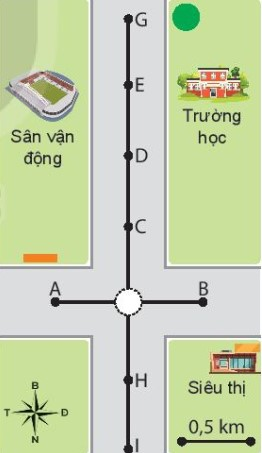
\includegraphics[width=0.25\linewidth]{../figs/VN10-2022-PH-TP005-1.jpg}
		\end{center}
	}
	\hideall
	{
		Sau 3 phút người đó đi được quãng đường là:
		
		$$s = vt = \SI{1,5}{km}.$$ 
		
		Như vậy người đó đến vị trí điểm E.
	}

	
	\item \mkstar{2}
	
	{
		
		Một ô tô chạy liên tục, trong 2 giờ đầu với tốc độ $\SI{80}{km/h}$, trong 1 giờ sau chạy với tốc độ $\SI{50}{km/h}$. Tốc độ trung bình của xe trong cả quá trình là bao nhiêu?
	}
	\hideall{
		
		Đoạn đường đi được trong 2 giờ đầu
		
		$$s_1 = v_1 t_1.$$
		
		Đoạn đường đi được trong 1 giờ sau
		
		$$s_2 = v_2t_2.$$
		
		Tốc độ trung bình của xe
		
		$$v_\text{tb} = \dfrac{s_1 + s_2}{t_1 + t_2} = \SI{70}{km/h}.$$
		
	}

\item \mkstar{2}

{
	
	Một người đi xe bắt đầu cho xe chạy trên đoạn đường thẳng: trong 10 giây đầu xe chạy được quãng đường $\SI{50}{m}$, trong 10 giây tiếp theo xe chạy được $\SI{150}{m}$. Tính tốc độ trung bình của xe máy trong khoảng thời gian nói trên.
}
\hideall{
	
	Tốc độ trung bình của xe máy
	
	$$v_\text{tb} = \dfrac{S_1 + S_2}{t_1 + t_2} = \SI{10}{m/s}.$$
}

	\item \mkstar{3}

{
	Một xe máy điện đi nửa đoạn đường đầu tiên với tốc độ trung bình $v_1 = \SI{24}{km/h}$ và nửa đoạn đường sau với tốc độ trung bình $v_2 = \SI{40}{km/h}$. Tính tốc độ trung bình trên cả đoạn đường.
	
}
\hideall{Gọi $2s$ là chiều dài cả đoạn đường.
	
	Thời gian đi nửa đoạn đường đầu:
	
	$$t_1 = \dfrac{s_1}{v_1} = \dfrac{s}{48}.$$
	
	Thời gian đi nửa đoạn đường cuối:
	
	$$t_2 = \dfrac{s_2}{v_2} = \dfrac{s}{80}.$$
	
	Tốc độ trung bình trên cả đoạn đường của xe máy điện:
	
	$$v = \dfrac{s}{t_1 + t_2} = \dfrac{s}{\dfrac{s}{48} + \dfrac{s}{80}} = \SI{30}{km/h}.$$
	
}

\item \mkstar{3}

{
	
	Một ô tô chạy trên đoạn đường thẳng từ A đến B phải mất khoảng thời gian $t$. Trong nửa đầu của khoảng thời gian này ô tô có tốc độ là $\SI{60}{km/h}$. Trong nửa khoảng thời gian cuối ô tô có tốc độ là $\SI{40}{km/h}$. Tính tốc độ trung bình trên cả đoạn AB.
}
\hideall{
	
	Tốc độ trung bình:
	
	$$v_\text{tb} = \dfrac{S}{t} = \dfrac{v_1\cdot\dfrac{t}{2}+v_2\cdot\dfrac{t}{2}}{t}=\dfrac{v_1 + v_2}{2} =\SI{50}{km/h}.$$		
}



\item \mkstar{3}

{
	
	Một người đi xe đạp từ A đến B với tốc độ $\SI{12}{km/h}$ trong $\dfrac{1}{3}$ quãng đường, và tốc độ $\SI{18}{km/h}$ trong $\dfrac{2}{3}$ quãng đường còn lại. Tính tốc độ trung bình của người đó trên cả đoạn đường AB.
}
\hideall{
	
	Thời gian đi $\dfrac{1}{3}$ quãng đường đầu:
	
	$$t_1 = \dfrac{S}{3v_1} = \dfrac{S}{36}.$$
	
	Thời gian đi $\dfrac{2}{3}$ quãng đường còn lại:
	
	$$t_2 = \dfrac{2S}{3v_2} = \dfrac{S}{27}.$$
	
	Tốc độ trung bình của người đó
	
	$$v_\text{tb} = \dfrac{S}{t_1 + t_2} = \dfrac{S}{\dfrac{S}{36} + \dfrac{S}{27}} \approx \SI{15,43}{km/h}.$$
}

\item \mkstar{3}

{
	
	Một chiếc thuyền cao tốc đi từ bến A đến bến B. Trong $\dfrac{2}{3}$ thời gian đầu tốc độ của thuyền là $v_1 = \SI{45}{km/h}$, thời gian còn lại thuyền chuyển động với tốc độ $v_2$ bằng bao nhiêu để tốc độ trung bình của nó trên cả quãng đường AB là $v = \SI{48}{km/h}$?
	
}
\hideall{
	
	Tốc độ trung bình của thuyền trên đoạn đường AB:
	$$v_\text{tb}=\dfrac{v_1\cdot\dfrac{2t}{3}+v_2\cdot\dfrac{t}{3}}{t}=\dfrac{2v_1}{3}+\dfrac{v_2}{3}\Rightarrow v_2=\SI{54}{\kilo\meter/\hour}.$$
}

\item \mkstar{3}\\
{	Một người đua xe đạp đi trên $\dfrac{1}{3}$ quãng đường đầu với tốc độ $\SI{25}{km/h}$. Tính tốc độ của người đó đi trên đoạn đường còn lại. Biết rằng tốc độ trung bình trên cả đoạn đường là $v_\text{tb} = \SI{20}{km/h}$.
}
\hideall{
	Tốc độ trung bình trên cả đoạn đường
	$$v_\text{tb}=\dfrac{s}{\dfrac{s}{3v_1}+\dfrac{2s}{3v_2}}=\dfrac{1}{\dfrac{1}{3v_1}+\dfrac{2}{3v_2}}$$
	$$\Leftrightarrow 20=\dfrac{1}{\dfrac{1}{3\cdot25}+\dfrac{2}{3v_2}}\Rightarrow v_2=\SI{18.18}{\kilo\meter/\hour}.$$
}




	\item \mkstar{3}\\
	{Một ô tô đi trên quãng đường AB với tốc độ trung bình $\SI{54}{km/h}$. Nếu giảm tốc độ trung bình đi $\SI{9}{km/h}$ thì ôtô đến B trễ hơn dự định 45 phút. Tính quãng đường AB và thời gian dự tính để đi quãng đường đó.
	}
	\hideall{Gọi $t$ là thời gian dự định để đi quãng đường AB, $v$ là tốc độ trung bình ban đầu và $s$ là chiều dài quãng đường AB. Phương trình chuyển động cho các trường hợp đi đúng tốc độ trung bình dự kiến và đi chậm hơn lần lượt là 
		\begin{equation}
			\label{eq:1}
			s=vt=54t
		\end{equation}
	\begin{equation}
		\label{eq:2}
		s=\left(v-9\right)\left(t+\SI{0.75}{}\right)=45\left(t+\SI{0.75}{}\right)
	\end{equation}
		Từ phương trình (\ref{eq:1}) và phương trình (\ref{eq:2}), giải được $t=\SI{3,75}{\hour}$.	\\
		Chiều dài quãng đường AB: $s=54t=\SI{202.5}{\kilo\meter}$.
		
	}

\item \mkstar{3}

{
	Một cậu bé dắt chó đi dạo về nhà, khi còn cách nhà $\SI{10}{m}$, con chó chạy về nhà với tốc độ $\SI{5}{m/s}$. Vừa đến nhà nó lại chạy ngay lại với tốc độ $\SI{3}{m/s}$. Tính tốc độ trung bình của chú chó trong quãng đường đi được kể từ lúc chạy về nhà đến lúc gặp lại cậu bé, biết cậu bé đi đều với tốc độ $\SI{1}{m/s}$.
}
\hideall{
	
	Thời gian chú chó về đến nhà là
	
	$$t_1 = \dfrac{s_1}{v_c} = \SI{2}{s}.$$
	
	Trong thời gian đó cậu bé đi được
	
	$$s_n = t_1 v_n = 1 \cdot 2 = \SI{2}{m}.$$
	
	Khoảng cách từ cậu bé đến nhà lúc đó là
	
	$$s' = s - s_n = \SI{8}{m}.$$
	
	Thời gian chú chó chạy từ nhà tới lúc gặp lại cậu bé
	
	$$t_2 = \dfrac{s'}{v_c + v_n} = \SI{2}{s}.$$
	
	Chú chó đã quay lại một đoạn là:
	
	$$s_2 = v_ct_2 = 3 \cdot 2 = \SI{6}{m}.$$
	
	
	Tốc độ trung bình của chú chó trong cả quá trình là: 
	
	$$v_\text{tb} = \dfrac{s_1 + s_2}{t_1 + t_2} = \SI{4}{m/s}.$$
}

	
	\item \mkstar{3}
	
	{
		
		Một người đi xe máy chuyển động trên đường thẳng theo 3 giai đoạn: Giai đoạn 1 chuyển động với tốc độ không đổi $v_1 = \SI{30}{km/h}$ trong $\SI{10}{km}$ đầu tiên; giai đoạn 2 chuyển động với tốc độ $v_2 = \SI{40}{km/h}$ trong 30 phút; giai đoạn 3 chuyển động trên đoạn đường $\SI{4}{km}$ trong 10 phút. Tính tốc độ trung bình trên cả đoạn đường.
	}
	\hideall{
		
		Thời gian xe máy chuyển động giai đoạn đầu
		
		$$t_1 = \dfrac{s_1}{v_1} = \dfrac{1}{3}\ \text{h}.$$
		
		Quãng đường giai đoạn sau:
		
		$$s_2 = v_2t_2 = \SI{20}{km}.$$
		
		Ta có:
		
		$$s = s_1 + s_2 + s_3 = \SI{34}{km}.$$
		
		$$t = t_1 + t_2 + t_3 = \SI{1}{h}.$$
		
		Tốc độ trung bình của xe máy trên cả đoạn đường:
		
		$$v_\text{tb} = \dfrac{s}{t} = \SI{34}{km/h}.$$
		
	}

	

	\item \mkstar{3}
	
	{
		Một ô tô chuyển động trên đoạn đường MN. Trong một phần hai quãng đường đầu đi với $v = \SI{40}{km/h}$. Trong một phần hai quãng đường còn lại đi trong một phần hai thời gian đầu với $v = \SI{75}{km/h}$ và trong một phần hai thời gian cuối đi với $v = \SI{45}{km/h}$. Tính tốc độ trung bình trên đoạn MN.
	}
	\hideall{
		
		Tốc độ trung bình trong nữa quãng đường cuối:
		$$v_\text{tb 2}=\dfrac{v_2\cdot\dfrac{t}{2}+v_3\cdot \dfrac{t}{2}}{t}=\dfrac{v_2+v_3}{2}=\SI{60}{\kilo\meter/\hour}$$
		Tốc độ trung bình trên cả đoạn đường:
		$$v_\text{tb}=\dfrac{s}{\dfrac{s}{2v_1}+\dfrac{s}{2v_\text{tb 2}}}=\dfrac{2}{\dfrac{1}{v_1}+\dfrac{1}{v_\text{tb 2}}}=\SI{48}{\kilo\meter/\hour}.$$
	}
	
	\item \mkstar{3}
	
	{
		
		Một người đi xe máy trên một đoạn đường thẳng AB. Trên một phần ba đoạn đường đầu đi với $v_1 = \SI{30}{km/h}$, một phần ba đoạn đường tiếp theo với $v_2 = \SI{36}{km/h}$ và một phần ba đoạn đường cuối cùng đi với $v_3= \SI{48}{km/h}$. Tính $v_\text{tb}$ trên cả đoạn AB.
		
	}
	\hideall{
		
	Tốc độ trung bình trên của đoạn đường AB:
	$$v_\text{tb}=\dfrac{s}{\dfrac{s}{3v_1}+\dfrac{s}{3v_2}+\dfrac{s}{3v_3}}=\dfrac{3}{\dfrac{1}{v_1}+\dfrac{1}{v_2}+\dfrac{1}{v_3}}=\SI{36.61}{\kilo\meter/\hour}.$$
	}
\end{enumerate}